\documentclass[12pt]{article}
\usepackage[utf8]{inputenc}
\usepackage{csquotes}
\usepackage[spanish]{babel}
\usepackage{graphicx}
\usepackage[style=apa]{biblatex}
\addbibresource{references.bib}
\usepackage[hidelinks]{hyperref}
\usepackage[left=3cm, right=3cm, top=2cm]{geometry}
\usepackage{subcaption}

\newcommand{\HRule}{\rule{\linewidth}{0.5mm}}
\title{\textbf{\huge Reconocimiento automático de notas del piano: Una comparación entre RNAs, MSVs y ADs}}
% \title{\textbf{\huge Automatic recoginition of piano notes: A comparison between ANNs, SVMs and DTs}}
\author{{David Rodríguez Bacelar} \\[0.25cm] {Kevin Millán Canchapoma} \\[0.25cm]{Luca D'angelo Sabín} \\[0.25cm]{Jorge Hermo González}}
\date{\today}

\begin{document}

\maketitle
\HRule
\bigskip\bigskip\bigskip\bigskip\bigskip\bigskip
\begin{figure}[h!]
	\centering
	
\includegraphics[height=180px]{udc.jpg}
	\label{fig:diagram1}
\end{figure}

\newpage

\tableofcontents

\newpage
\section{Introducción}

A raíz de la pandemia, el aumento del interés por el aprendizaje en diferentes ámbitos llegó tambíen a la música, y con él, la aparición
de herramientas para aprender a tocar diferentes instrumentos de forma autodidacta.

\bigskip
Así, para cualquiera que esté aprendiendo, el escuchar una canción que te gusta e intentar tocarla es algo que acaba siendo un proceso
frustante y que requiere una gran cantidad de horas intentando sacar las notas que la componen.

\bigskip
Nuestro sistema se encargaría entonces de reconocer y diferenciar a partir de audios las notas de una pieza de piano
pudiendo, en un futuro, ser capaz de detectar acordes y tonalidades, siendo útil en aplicaciones como Spotify, Tidal... Para ello, haremos uso
de diferentes técnicas de aprendizaje automático como las redes de neuronas artificiales, árboles de decisión y máquinas de soporte vectorial,
comparando su rendimiento y eligiendo la que mejor resultados nos ofrezca.

\bigskip
A lo largo de esta memoria analizaremos a fondo el problema a resolver en la Sección \ref{Descripción del problema}, desarrollaremos las diferentes soluciones en la
Sección \ref{Desarrollo}, hablaremos sobre las conclusiones del trabajo en la Sección \ref{Conclusiones} y finalizaremos comentando las aplicaciones al mundo
real en la Sección \ref{Trabajo futuro}. También se podrá consultar las bibliografía utilizada en la Sección \ref{Análisis bibliográfico} y \ref{Bibliografía}.

\subsection{Glosario}
\label{Glosario}
\begin{itemize}
	\item Sample: muestra de carácter musical
	\item Cover: Reinterpretación de una canción por parte de alguien diferente al que la compuso.
	% \item TF: transformada de Fourier
\end{itemize}

\newpage

\section{Descripción del problema}
\label{Descripción del problema}

Nuestro sistema se centrará en reconocer, a partir de un audio, la nota del piano que se está tocando. Escogimos este instrumento por la cantidad de recursos
que podemos encontrar y por su naturaleza invariable al ser tocada por una u otra persona.

\bigskip
Dada la naturaleza de nuestro sistema, descartamos utilizar la especificidad o la sensibilidad ya que nos es indiferente las clases en las que se clasifiquen
las notas (el coste de un falso positivo o un falso negativo es el mismo).

\bigskip
Así, como solo nos interesa una correcta clasificación global, pensamos en utilizar la precisión, la cual sigue la fórmula:

\begin{equation}
	Precision = \frac{VN + VP}{(VN + FN + VP + FP)}
\end{equation}

\smallskip
El incoveniente de esta métrica está en que si tenemos un conjunto de patrones desbalanceado (gran diferencia en el número de
patrones positivos y negativos), la precisión podría alcanzar valores muy altos con sistemas que clasifiquen todos los patrones en la clase con mayor número de ellos
en el entrenamiento.

\bigskip
La métrica que utilizaremos entonces para valorar los resultados obtenidos y que palia los problemas
mencionados anteriormente será la \textbf{F1 score}. Esta se corresponde con la media armónica de la sensibilidad y el
valor predictivo positivo y está caracterizada por la fórmula: 

\begin{equation}
	F1 = \left(\frac{Sensibilidad^{-1} + VPP^{-1}}{2}\right)^{-1}
\end{equation}

donde, 
\begin{equation}
	Sensibilidad = \frac{VP}{(FN + VP)}
\end{equation}

\begin{equation}
	VPP = \frac{VP}{(VP + FP)}, 
\end{equation}

\smallskip
Quizá el único inconveniente de esta métrica es su difícil interpretación, más allá de comparar los valores que ofrecen diferentes sistemas.
El valor más alto que puede alcanzar es de 1 (todos los patrones se clasificaron correctamente) y el más bajo es de 0 (todos los patrones se clasificaron
incorrectamente). 

\subsection{Restricciones}
\bigskip
Como única restricción, en dicho audio solo puede haber una nota sonando a la vez para que el sistema sea capaz de reconocerla correctamente.

\subsection{Características}
\bigskip
La base de datos con la que contamos tiene un total de 5.406 audios con una media de más de 50 \textit{samples} por cada una de las 85 notas del piano (a partir de \textit{C1}), tocadas
desde posiciones e intensidades distintas y grabadas con micrófonos diferentes. Dichos \textit{samples} están en formato \textit{.wav} en estéreo, con un 
\textit{bitrate} de \textit{2304kbps}, \textit{24 bits per sample} y un \textit{sample rate} de \textit{48kHz}. Todo ello ocupa un total de \textit{34.5GB} en disco.
La duración media de los \textit{samples} es de aproximadamente xxx s.

\bigskip
El origen de la base de datos es una librería de piano de la compañía \textit{FluffyAudio} \textit{\url{https://www.fluffyaudio.com/shop/scoringpiano/}} 
grabada en 2016 y pensada para jazz, música clásica y bandas sonoras.

\section{Análisis bibliográfico}
\label{Análisis bibliográfico}
Para profundizar en el tema antes de abordarlo, en esta sección se analizan diferentes artículos científicos relacionados con la inteligencia
artificial y el reconocimiento de audio, ya sea específicamente relacionado o no con el mundo del reconocimiento de piezas o notas musicales.

\bigskip
Trabajos como el de \cite{osmalsky2012neural} nos aportan nuevos enfoques, 
en el que, en lugar de detectar las notas por separado, analizan todo el espectro de frecuencias para poder reconocer acordes completos de diferentes instrumentos;
utilizan una técnica llamada Pitch Class Profile (PCP), que obtiene las relaciones energéticas de cada nota en la escala a partir de un audio.

\bigskip
Además, como resumen \cite{benetos2018automatic},
a pesar del estado avanzado de la transcripción automática de canciones, aún están presentes retos tales como la independencia de los intrumentos, de los estilos
musicales o la interpretación de la expresividad.

\bigskip
Otros trabajos mas antiguos como los de \cite{foo1999recognition}, describen un algoritmo capaz de reconocer notas
de un piano a partir de piezas sintetizadas o acústicas, que son digitalmente muestreadas y transformadas al dominio de frecuencia usando 
la transformada de Q constante a partir de la cual se la aplican diferentes técnicas para identificar las notas.

\bigskip
En un terreno más general, trabajos como el de \cite{chang2017audio}, exploran la identificación de \textit{covers} utilizando
estructuras más novedosas que no desarrollaremos en este trabajo como son las Redes de Neuronas Convolucionales. Las salidas de este
sistema corresponderían con la probabilidad de ser una \textit{cover} (comparándola con la canción original), y se ordenarían por dicha 
probabilidad elaborando un ranking.

\bigskip
===MEJORAR===
También encontramos la tesis de \cite{klapuri2004signal} que propone un sistema capaz de generar una representación 
simbólica a partir de un audio. centrandose en el desarrollo de los algoritmos que pueden ser usados para detectar sonidos harmónicos y señales polifónicas

\bigskip
El uso de redes de neuronas artificiaes también están presentes en trabajos como \cite{solanki2019music}, que aborda la identificación de
los instrumentos que forman part de piezas polifónicas. Utiliza una red de neuronas convolucional de 8 capas y se apoya en los espectrogramas 
MEL para mapear datos del audio.

\bigskip
Para finalizar, ya en un campo algo más alejado del musical, podemos destacar el trabajo elaborado por \cite{baevski2021unsupervised},
el cual profundiza en el campo de reconocimiento del habla mediante inteligencia artificial.
A diferencia de otros sistemas de reconocimiento, este trabajo no usa datos etiquetados que limiten el reconocimiento a un grupo reducido de idiomas. 
Esta técnica necesita menos requerimientos, aprovechando representaciones auto supervisadas del habla para segmentar el audio y aprender a 
mapear desde estas representaciones a fonemas via \textit{Adversarial Training}.

\bigskip

\newpage
\section{Desarrollo}
\label{Desarrollo}
Para el desarrollo de este sistema utilizaremos un método basado en aproximaciones, es decir, comenzaremos acotando el problema e iremos aumentando
la complejidad a medida que obtenemos resultados satisfatorios.
\subsection{Primera aproximación}
\label{Primera aproximación}

\subsubsection{Descripción}
En esta primera aproximación nos limitaremos a diferenciar únicamente entre dos notas. 
Escogimos las notas \textit{C4} y \textit{A5} de los cuales usaremos 92 y 56 audios de cada una, respectivamente.

\begin{figure}[h!]
	\centering
	\begin{subfigure}{.5\textwidth}
		\centering
		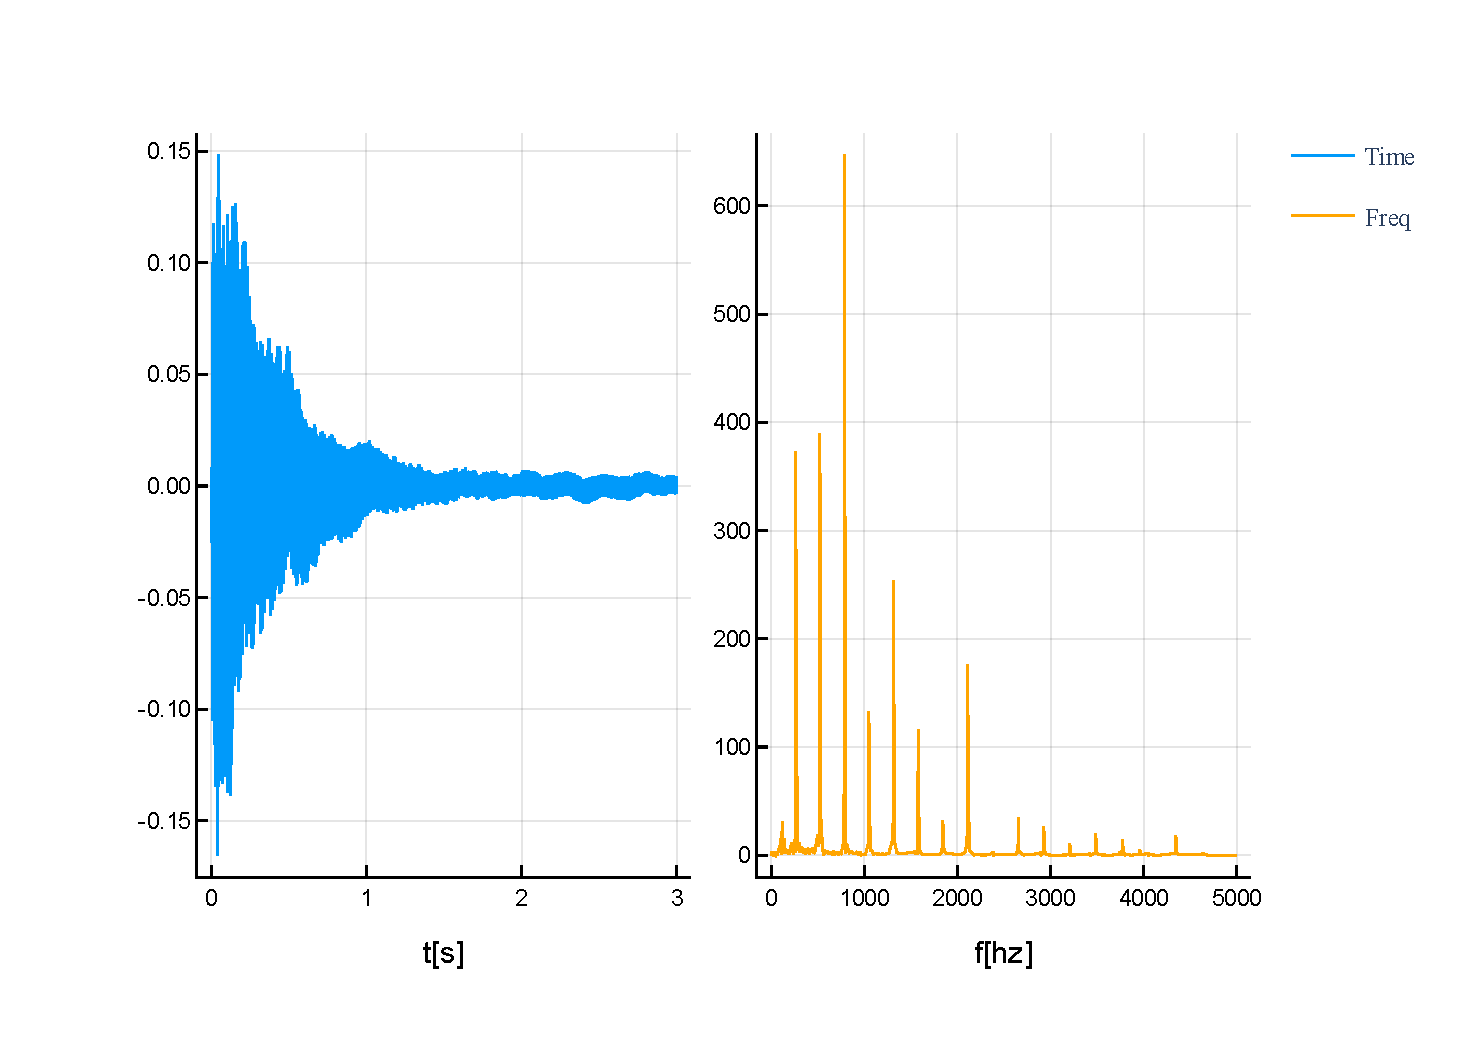
\includegraphics[width=1.0\linewidth]{c4.pdf}
		\caption{C4}
		\label{fig:sub1}
	\end{subfigure}%
	\begin{subfigure}{.5\textwidth}
		\centering
		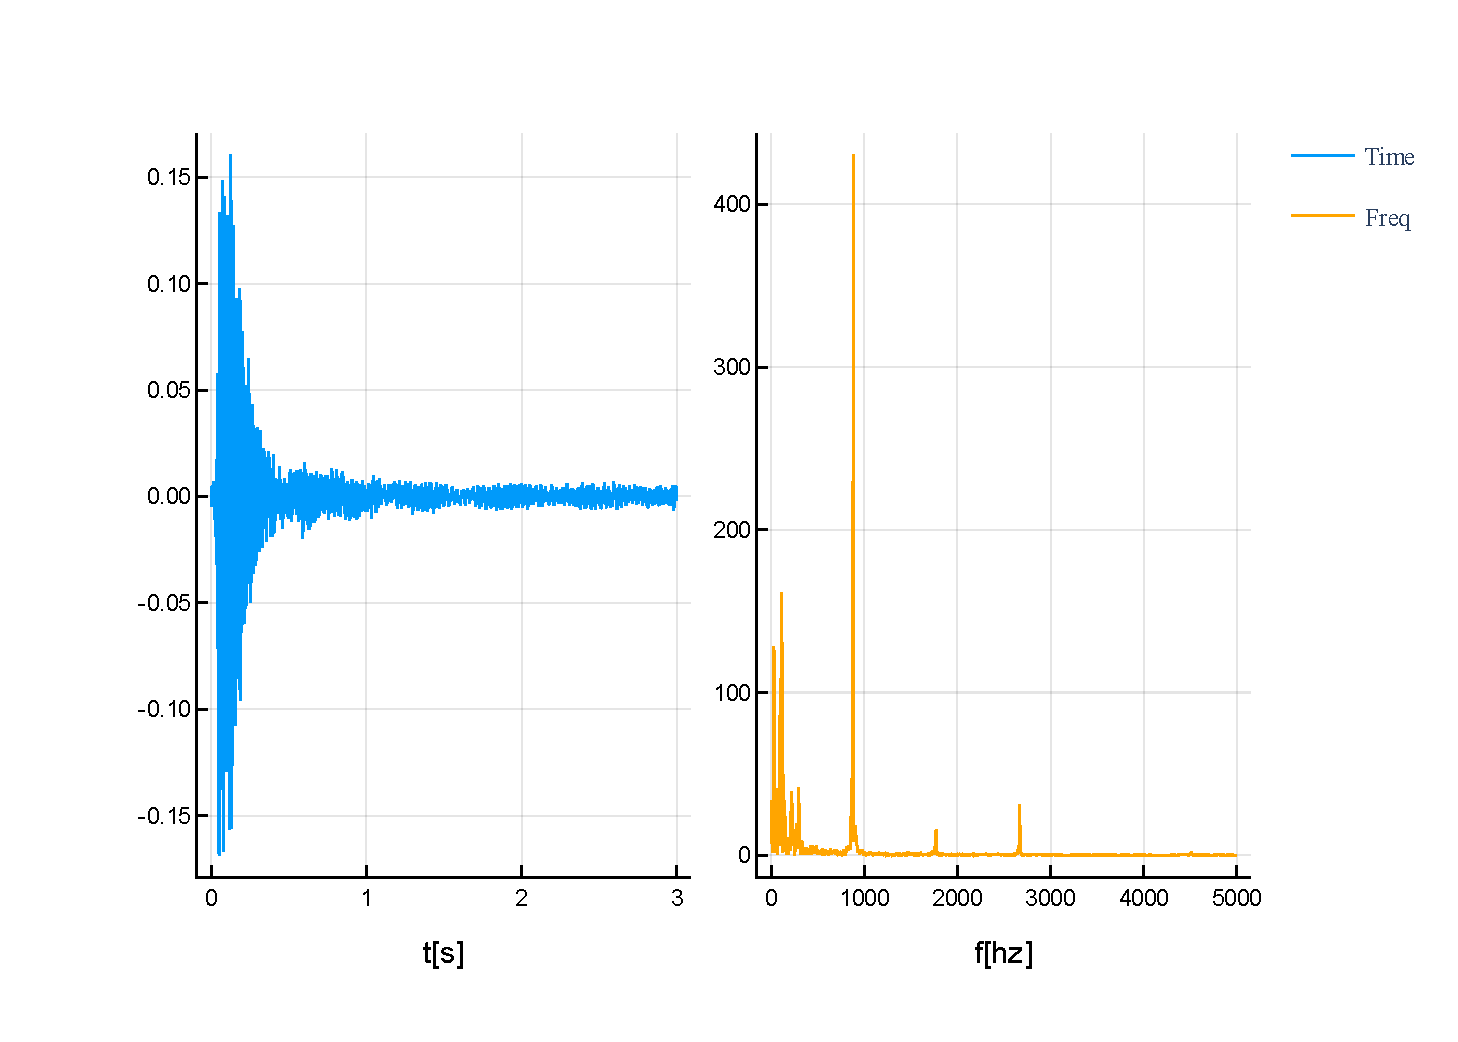
\includegraphics[width=1.0\linewidth]{a5.pdf}
		\caption{A5}
		\label{fig:sub2}
	\end{subfigure}
\end{figure}

\bigskip
Dado que cada muestra tiene una duración diferente, decidimos quedarnos solo con los 3 primeros segundos de cada audio (que es donde está la información más
relevante de la nota) y, para la frecuencia, acotaremos cada señal entre 0 y 5000 Hz. Ya que la frecuencia máxima que se alcanza en el 
piano clásico es de 4186 Hz (\textit{C8}) y la más baja, en nuestra base de datos, es de 32.7Hz (\textit{C1}), escogimos un rango
de frecuncias ampliado debido a que es posible que exista información que nos ayude a identificar la nota.

\bigskip
Además, como las notas de un mismo instrumento se diferencian principalmente por la frecuencia (una nota más aguda tiene una mayor frecuencia
y una más grave, una menor), calcularemos de las señales en el dominio del tiempo su relación en el dominio de la frecuencia utilizando la
Transformada de Fourier y, posteriormente, extraeremos las siguientes características:
\begin{itemize}
	\item \textbf{Energia media de la señal}: ya que las señales con más frecuencia (más agudas) tienen más energía, esta característica nos podría
		ayudar a diferenciar entre notas tocadas con la misma intensidad.
	\item \textbf{Media, desviación tipica, y valor máximo de la frecuencia en intervalos no uniformes}: la frecuencia de cada nota
		aumenta de forma exponencial siguiendo la fórmula:

		\begin{equation}
			f_{i+1} = f_{i}\cdot(\sqrt[12]{2}), f_0 = 27.5 Hz
		\end{equation}

		Por ello decidimos dividir el espectro en 10 intervalos de longitud variable siguiendo dicha distribución. 
		Podríamos entonces obtener un intervalo donde la media y la desviación típica de la frecuencia fueran más elevados que el resto,
		ayudándonos a identificar la nota.
		
		Los intervalos que usaremos son los siguientes:
		
		\textit{(0.0, 380.3), (380.3, 783.21), (783.21, 1210.08), (1210.08, 1662.33),\newline
		(1662.33, 2141.47), (2141.47, 2649.11), (2649.11, 3186.93), (3186.93, 3756.73), 
		(3756.73, 4360.42), (4360.42, 5000.0)}
	\item \textbf{Zero-crossing/s}: esta característica determina las veces que la señal, en el dominio del tiempo, toma el valor 0 cada segundo.
		Como dicha cracterística nos proporcionaría valores similares a la frecuencia media de la señal, podría contribuír a su correcta clasificación.
\end{itemize}

\section{Conclusiones}
\label{Conclusiones}

\section{Trabajo futuro}
\label{Trabajo futuro}

\section{Bibliografía}
\label{Bibliografía}
\printbibliography

\end{document}
